\documentclass{beamer}




\usetheme{Copenhagen}

\author{Juli\'{a}n Hern\'{a}ndez, Rodrigo Ipince, Jos\'{e} Mu\~{n}iz} 
\title{A Comparison of Three Algorithms for Building ST-Histograms} 
\institute{MIT} 

\begin{document}

	\begin{frame}
		\maketitle
	\end{frame}
	
	

	%
	%Slide 1:
	% How do we use histograms?
	%
	\begin{frame}
		\frametitle{Histograms in Postgres}�
			\begin{itemize}
				\item One dimensional 
				\item Independence assumption between fields in the same and different
					tables
			\end{itemize}
			
    				\begin{center}
					\texttt{SELECT * FROM students WHERE� age $\leq 19$ }
				\end{center}
		
		\begin{columns}[T]
		
  			\begin{column}{0.4\textwidth}
			   	\begin{center} 
					  \only<1>{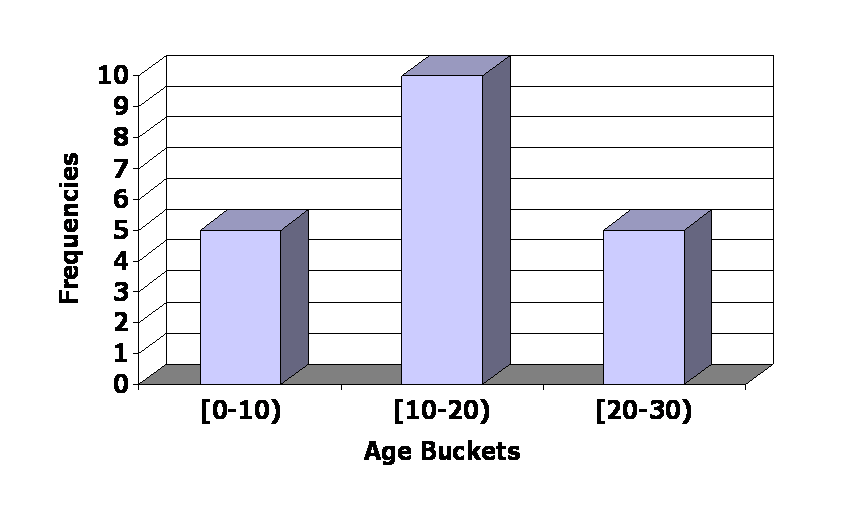
\includegraphics[width=130pt]{RegHistogram.PNG}}
					  \only<2-3>{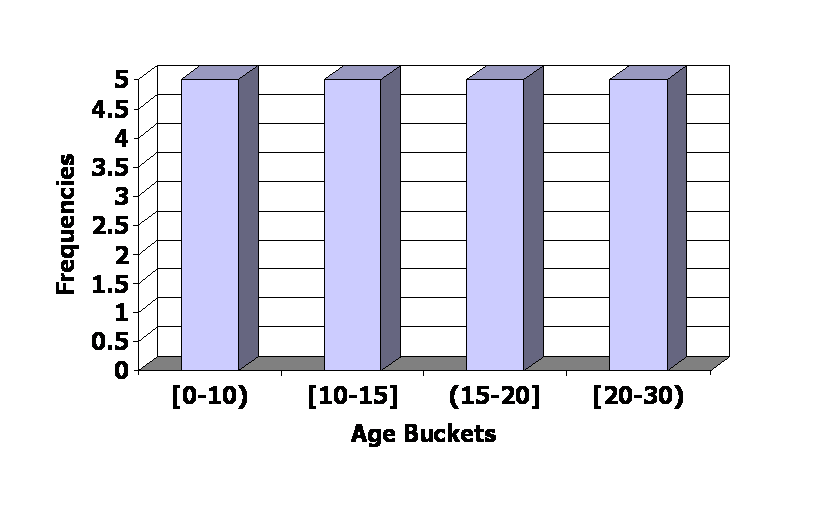
\includegraphics[width=130pt]{PostgresHist.PNG}}
					  \only<4-5>{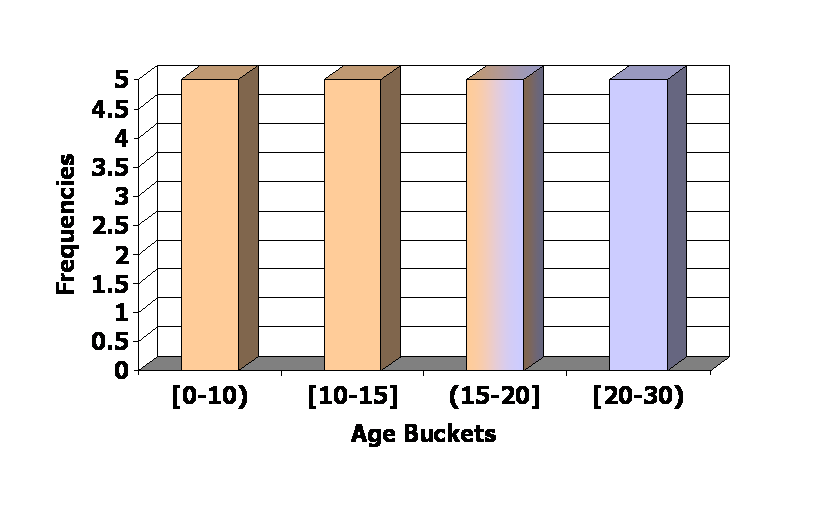
\includegraphics[width=130pt]{PostgresHistSel.PNG}}
				\end{center} 

		   	\end{column}

			 \begin{column}{0.4\textwidth}	
			   	\begin{center} 
					 \only<3-4>{ 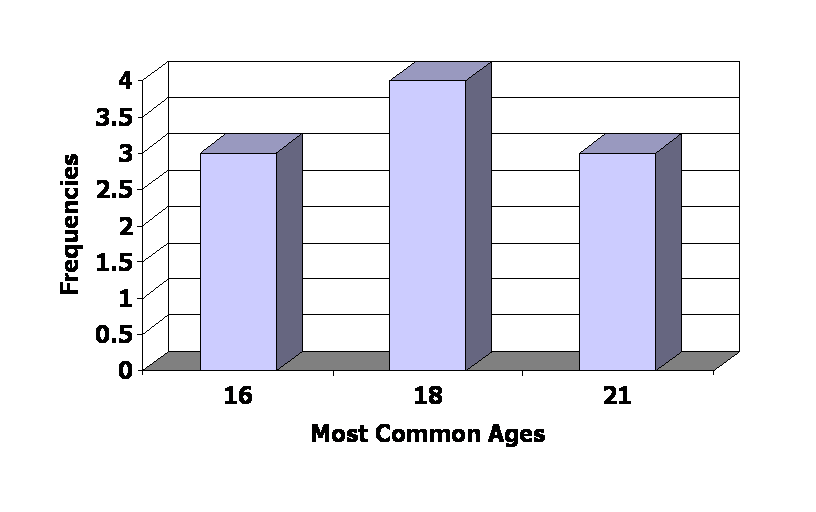
\includegraphics[width=130pt]{CommonAges.PNG} }
					 \only<5>{ 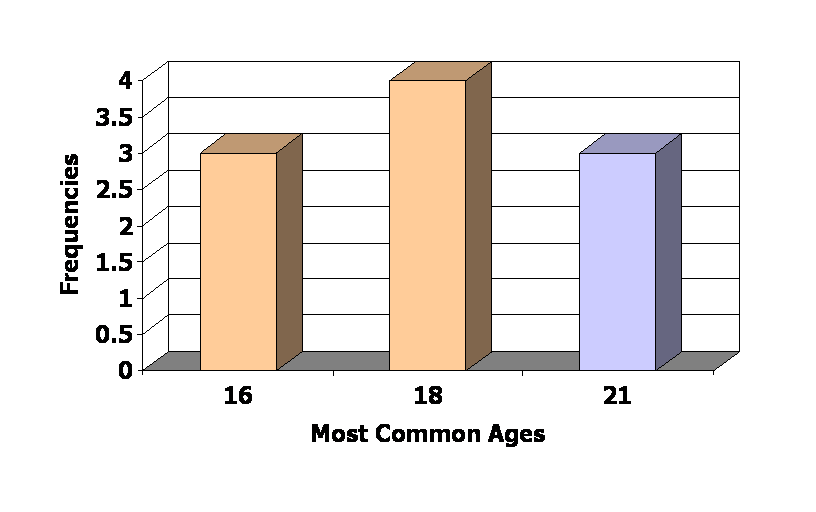
\includegraphics[width=130pt]{CommonAgesSel.PNG} }
				\end{center} 

			 \end{column}
		\end{columns}

		\bigskip
		
		\only<5>{$$\sigma = \alpha \times \sigma_{hist}� + \beta \times \sigma_{MCV} $$}
		
	\end{frame}	


	%
	%Slide 2:
	% How do we build histograms?
	%
	\begin{frame}
		  \frametitle{Building histograms: Traditional cost-based optimization}
		
		\begin{columns}[T]
  			\begin{column}{0.3\textwidth}
    				Four components: 
    				\begin{itemize}
				      \item Optimizer
				      \item Executor
				      \item Histogram
				      \item Statistics gatherer
				\end{itemize}
		   	\end{column}

			 \begin{column}{0.7\textwidth}	
				 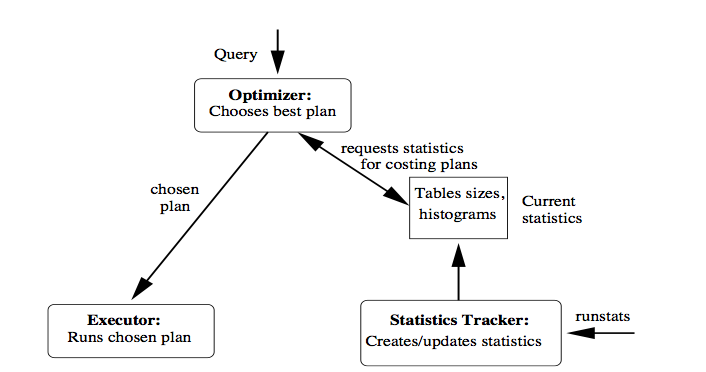
\includegraphics[width=200pt]{TraditionalPlan.PNG} 

			 \end{column}
		\end{columns}

			\bigskip
			
			No connection between executor and histogram. 
			

			
	\end{frame}	

	
	%Slide 3: 
	% Problems with model
	\begin{frame}
	
		\frametitle{Some problems with traditional approach}�	
			Key assumptions
			\bigskip 
			
			\begin{itemize}
				\item Uniformity of attribute values
				\item Uniformity of queries
				\item Constant number of records per block
				\item Random placement \emph{or} full page scan
			\end{itemize}
			
			\bigskip
			
			Problems: 
			\begin{itemize}
				\item Tradeoff between performance cost of statistics gatherer 
					versus adaptability to change of conditions  
				\item Tradeoff between number of pages read and adaptability
					to correlated data
				\item Postgres suggests turning off \texttt{autovacuum} 
					for large tables and running end-of-day analysis.  
			\end{itemize}			
		
	\end{frame}


	%Slide 4: 
	% Solution : ST-Histograms
	\begin{frame}
	
		\frametitle{Self Tuning Histograms}�	
			

				Can we do something without needing to implement multidimensional histograms?

				\bigskip 
				
				 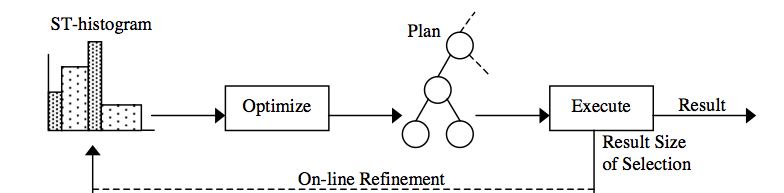
\includegraphics[width=300pt]{STModel.PNG} 
			
		\pause 
		{Interface}
				\begin{itemize}
				\item Executor executes \\
					~~\texttt{emit([a...b], val)}
				\item Histogram builder provides \\
					~~\texttt{int estimate([a...b])}
				\end{itemize}
			
	
	\end{frame}


	%Slide 5: 
	% Some details
	\begin{frame}
	
		\frametitle{Self Tuning Histograms: Interface and Motivation}�	

		\begin{itemize}
			\item {How do we build the histogram without looking at data?}
				\begin{itemize}
					\item Update frequencies
					\item Update buckets
				\end{itemize}
				
			\item{First idea: Uniform blame}
				\begin{itemize}
					\item Nothing known: assume uniform distribution
					\item \emph{Update frequencies: } \\
						 On \texttt{emit}, calculate percentage error $e$, 
						 multiply all affected intervals by $\alpha \times p \times e$,
						 where $p$ is frequency proportion. 
					\item \emph{Update buckets: } \\
						Split buckets with large frequencies. \\ 
						Merge buckets with small frequencies. 
						   
				\end{itemize}
		\end{itemize}

	\end{frame}


	\begin{frame}
	
		\frametitle{Updating frequencies}�	

			Result from \texttt{emit([0,19], 30)}
			
			 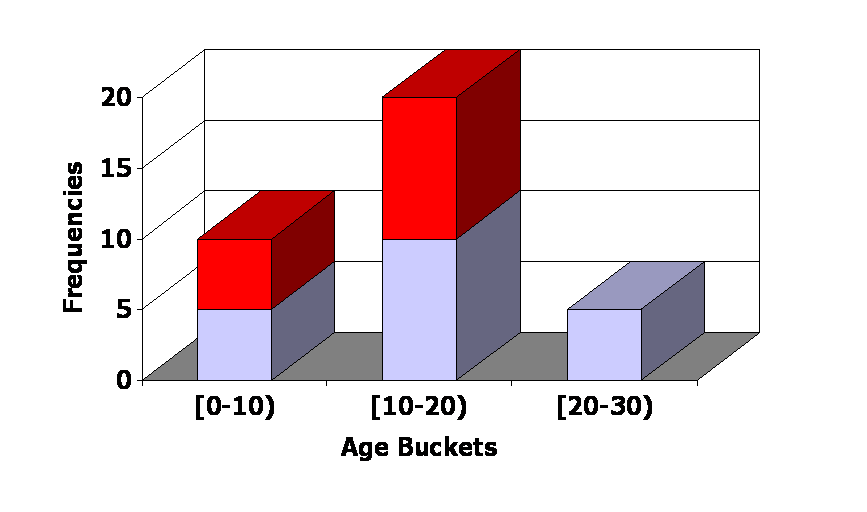
\includegraphics[width=300pt]{emit0-19-30.PNG} 

				
	\end{frame}
	


	\begin{frame}
	
		\frametitle{Merge and split}�	

			
			 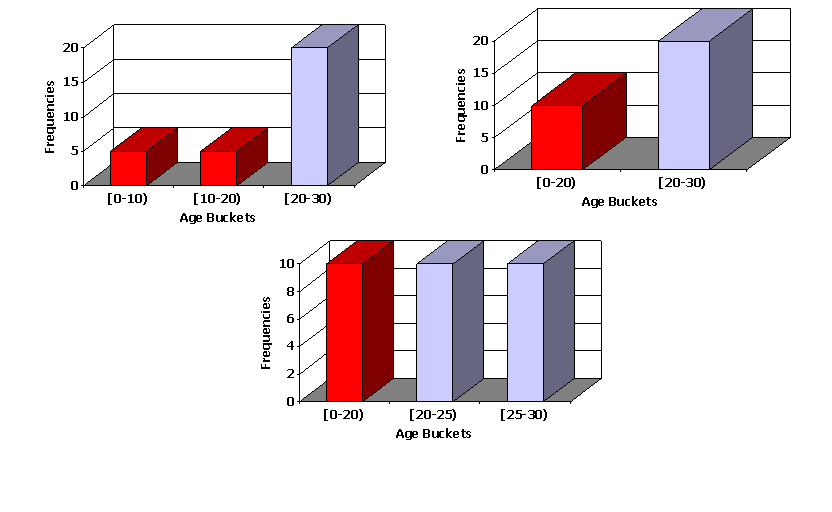
\includegraphics[width=300pt]{merge-split.PNG} 

				
	\end{frame}
	



	%Slide 6: 
	% Algorithm I
	\begin{frame}
	
		\frametitle{Improvements and alternatives}�	

		\begin{itemize}
			\item Occasionally renormalize data to fit to total number of tuples.\\
				\emph{Improves determination of error vs insertion}

			\item Adjust blame proportional to range and frequency
			\item Split most frequently updated ranges
		\end{itemize}
				
	\end{frame}
	
	
	
		
	
	
	%Slide 6:
	%Experimental Setup
	\begin{frame}
	
		\frametitle{Experimental Setup}�	

		
		\begin{itemize}
			\item Middle layer between PostgreSQL and end user
			\item Process: 
				\begin{enumerate}
					\item Relay query to Postgres
					\item Obtain query plan via \texttt{EXPLAIN}
					\item Simulate query, using results for calling \texttt{emit}
					\item Calculate error rate in generated histograms
				\end{enumerate}
			
		\end{itemize}
	 \end{frame}
	
	%Slide 8:
	%Results 
	\begin{frame}
	
		\frametitle{Results}�	

		
		\begin{itemize}
			\item Fast to adapt 
			\item Minimal insertion overhead (Small amount of tuples per query)			
				\begin{itemize}
					\item Ideal for large databases with constant insertions
						and varying ranges. 
				\end{itemize}
		\end{itemize}

		\bigskip

		Caveats: 
		\begin{itemize}
			\item Major optimizer misses due to independence assumptions,
				and not failures in row estimates. 
			\item Not all cases lead to performance gains. 
			\item No solution for \texttt{LIKE} queries.  
			 
		\end{itemize}
				

		
	\end{frame}
	
	

	
 
\end{document}